\section{مقدمه}

فرآیندهای همگام سازی در سیستم عصبی نقش مهمی دارند؛ به عنوان مثال، در زمینه پردازش اطلاعات و کنترل حرکتی. 
با این حال، همگامیِ بیش از حدِ طبیعی و کمتر از حدِ طبیعی باعث بروز اختلال در الگوی فعالیت نوسانی نواحی مختلف مغز می‌شود و عملکرد مغز را به شدت مختل می‌کند و مشخصه بسیاری از بیماری‌ها و اختلالات عصبی می‌باشد.
%با این حال، همگامی بیش از حد ممکن است عملکرد مغز را به شدت مختل کند و مشخصه بسیاری از اختلالات عصبی همین همگامی بیش از حد و ناهنجار است.
اختلالات عصبی متعددی، مانند پارکینسون، صرع، لرزش اساسی
\LTRfootnote{Essential Tremor (ET)}
 و وزوز گوش
\LTRfootnote{Tinnitus}
  ، با همگامی قوی و غیرعادی فعالیت نورون‌ها مشخص می‌شوند. کاهش نوسانات همگامِ غیرعادی در این بیماران با بهبود علائم بیماری همراه است 
\cite{uhlhaas2006neural}
.
%برای مثال کاهش نوسانات باند بتا به کمک داروها دوپامینرژیک یا تحریک عمیق مغز با فرکانس بالا با بهبود علائم حرکتی در بیماران پارکینسونی ارتباط مثبت دارد. 
%اختلالات مغزی متعددی مانند بیماری پارکینسون، لرزش اساسی، صرع و وِزوِز گوش با همگامی غیر طبیعی نورون ها همراه هستند.
 به عنوان مثال، در پارکینسون همگامی بیش از حد در ناحیه بیزل گانگلیا\LTRfootnote{Basal ganglia}
  با اختلالات حرکتی همراه است
 \cite{hammond2007pathological}
 ، در حالی که نورون‌ها در شرایط فیزیولوژیکی به صورت ناهمگام آتش می‌کنند.  کاهش نوسانات همگام در فرکانس‌های باند بتا (از ۸ تا ۳۵ هرتز) به کمک داروهای دوپامینرژیک با بهبود علائم حرکتی در بیماران پارکینسونی همبستگی مثبت دارد
  \cite{hammond2007pathological, kuhn2006reduction}.
  از طرف دیگر، تحریک هسته ساب تالامیک
\LTRfootnote{Subthalamic nucleus (STN)}
با فرکانس پایین (۵ تا ۲۰ هرتز)، که برای تقویت نوسانات همگام در همین فرکانس‌ها در نظر گرفته شده است منجر به وخامت بالینی قابل توجهی در علائم پارکینسون و عملکردهای حرکتی در انسان‌های بیمار و جوندگان پارکینسونی می‌شود
\cite{jenkinson2011new, moro2002impact, timmermann2004ten, eusebio2008effects, barnikol2008tremor, chen2011stimulation}.
در اختلال وزوز گوش نیز الگوهای غیر طبیعی افزایش فعالیت عصبی همگام در بیماران انسانی و مدل های جانوری مشاهده شده است
\cite{weisz2005tinnitus, weisz2007neural, dohrmann2007tuning, adamchic2014reversing}.
 به طور خاص، ریتم های عصبی پاتولوژیک بالاو مداوم در باند دلتا (۱/۵ تا ۴ هرتز) همچنین در فرکانس های باند گاما (بیشتر از ۳۰ هرتز) در بیماران مبتلا به وزوز گوش مزمن در مقایسه با افراد سالم دیده شد که با پریشانی مرتبط با وزوز گوش و بلندی وزوز گوش همبستگی دارد
 \cite{weisz2005tinnitus, weisz2007neural, lorenz2009loss}.
  علاوه بر این، یک ارتباط مثبت بین هنجارسازی این فعالیت‌های نورونی و کاهش شدت وزوز گوش وجود دارد
\cite{weisz2005tinnitus, weisz2007neural, dohrmann2007tuning, adamchic2014reversing, lorenz2009loss}.  
   روی هم رفته، همگامی غیر عادی فعالیت نورون‌ها می‌تواند به طور قابل توجهی فرآیندهای عصبی و عملکردهای مغزی را مختل کند و به عنوان یک هدف برای درمان های جدید بکار می‌رود.


امروزه درمان استاندارد برای بیماران پارکینسون مقاوم به درمان دارویی، تحریک عمیق مغز با فرکانس بالا
\LTRfootnote{High-frequency deep brain stimulation (HF-DBS)}
است. برای این منظور یک قطار پالس فرکانس بالا (بیشتر از ۱۰۰ هرتز) از طریق الکترودهایی که در عمق مغز کاشته شده است به قسمت‌های مشخصی از مغز اعمال می‌شود. درمان بیماری‌های عصبی و روانی شدید مانند پارکینسون، لرزش، درد خیالی و مزمن
\LTRfootnote{Chronic and phantom pain}
\footnote{درد فانتوم دردی است که در فقدان یک عضو از بدن درک می‌شود. فقدان عضو می‌تواند در نتیجه قطع عضو یا فقدان مادرزادی عضو باشد.}
، افسردگی اساسی
\LTRfootnote{Major depression disorder (MDD)}
، وسواس فکری و عملی
\LTRfootnote{Obsessive–compulsive disorder (OCD) }
%، سندروم توره
%\LTRfootnote{Tourette syndrome}
 و صرع به کمک تحریک عمیق مغز یک زمینه در حال رشد و امیدوار کننده است. با اینکه تا کنون مکانیزم‌های اثر تحریک عمیق مغز با فرکانس بالا کاملا شناخته نشده‌اند؛
%  چند مکانیزم دخیل در نتایج مشاهده شده
%%  از تحریک عمیق مغز با فرکانس بالا 
%  ممکن است مکانیزم مسدود کردن
%\LTRfootnote{Jamming}
%، مهار غشا، تحریک نورون‌های تحریکی و مهاری آوران
%\LTRfootnote{Afferent}
%، تحریک نورون‌های وابران
%\LTRfootnote{Efferent}
%، شکل پذیری دستگاه عصبی باشند
%\cite{benabid2005putative}.
مهمترین گزینه‌های نحوه اثر گذاری آن مکانیزم مسدود کردن
\LTRfootnote{Jamming}
و همچنین شکل پذیری دستگاه عصبی می‌باشد
\cite{benabid2005putative}.
%از نوشته دکتر ولیزاده برای طرح پژوهشی بنیاد نخبگان:

استفاده از مدل‌های محاسباتی برای شبیه‌سازی سلول‌های عصبی ناحیه‌ای از مغز 
%و برهمکنش آن‌ سلول‌ها با یکدیگر 
و همچنین شبیه‌سازی برهمکنش  بین مناطق مغزی مختلف امکان گسترش افق مراقبت‌های بالینی برای بیماری‌ها
% و شرایط عصبی 
 مختلف ایجاد می‌کند. برای مثال، اکثر تحریک‌های عمقی مغز از رهیافت حلقه‌باز\LTRfootnote{Open-loop}
استفاده می‌کنند که در آن تحریک با پارامترهای ثابت اعمال می‌شود. تأثیر متغیرهای کلیدی مانند منطقه هدف برای اعمال تحریک و شکل موج تحریک به طور دقیق شناخته نشده‌اند.
%، و در بررسی‌های مختلفِ اثربخشی طولانی مدت، نتایج متفاوتی دارد
تعریف دقیق پارامترهای شکل موج در تحریک عمقی مغز می‌تواند از آسیب دیدن بافت مغز یا الکترود جلوگیری کند، فعالیت عصبی را افزایش داده و هزینه انرژی را کاهش دهد که باعث افزایش عمر باتری می‌شود و از این رو از جراحی‌های جایگزینی دستگاه جلوگیری می‌شود. مدل‌های محاسباتی و شبیه‌سازی مدارهای مغزی می‌تواند در پیدا و بهینه کردن پارامترهای تحریک یاری دهنده باشند. بعلاوه شبیه‌سازی مدارهای مغزی امکان بررسی نشانگرهای زیستی مختلف را به ما می‌دهد که به کمک آن می‌توانیم یک مدل پیش‌بینی از نحوه پاسخِ سیستم عصبی به تحریک‌های مختلف بسازیم؛ سپس با درک نحوه اثرگذاری تحریک در نواحی مختلفِ مغز (روی فعالیت تک تک نورون ها و همچنین فعالیت جمعی آن ها) می‌توانیم روش‌های حلقه‌بسته‌ای\LTRfootnote{Closed-loop}
متناسب با هر بیمار طراحی کنیم. 

\section{نوسانات عصبی}
نوسان عصبی یا امواج مغزی، الگوهای ریتمیک یا تکراری فعالیت عصبی در سیستم عصبی مرکزی می‌باشند. بافت عصبی می‌تواند فعالیت‌های نوسانی را به طرق مختلف بوجود آورد.
%، که به وسیله مکانیسم درون نورون‌های فردی منفرد با تعامل بین نورون‌ها هدایت می‌شود.
 در یک نورون‌ تنها، نوسانات عصبی ممکن است به عنوان نوسان در پتانسیل غشا یا به عنوان الگوهای ریتمیک پتانسیل‌های عمل
 \LTRfootnote{Action Potential}
  باشند. در سطح جمعیت‌های نورونی، فعالیت هماهنگ تعداد زیادی از نورون‌ها می‌تواند به نوسانات ماکروسکوپی منجر شود که می‌تواند در نوار مغزی
 \LTRfootnote{Electroencephalogram}
  مشاهده شود. فعالیت‌های نوسانی در گروه‌های نورونی به‌طور کلی از ارتباطات بازخوردی بین نورون‌ها ناشی می‌شود. این ارتباطات منجر به هماهنگ شدن و همگام‌سازی الگوهای شلیک نورون‌ها می‌شود. علاوه بر این تعامل بین نورون‌ها می‌تواند باعث تولید فعالیت نوسانی در فرکانس‌هایی بیشتر از فرکانس شلیک یک نورون‌ تنها شود.
%  یک مثال شناخته شده از نوسانات مغناطیسی عصبی فعالیت آلفا است. 
  
%  نوسان‌های عصبی توسط محققان در اوایل سال ۱۹۲۴ (توسط هانس برگر) مشاهده شد. بیش از ۵۰ سال بعد، رفتار نوسانی ذاتی در عصب‌های ستون مهره داران مشاهده شد، اما نقش عملکردی آن هنوز کاملاً درک نشده‌است. فعالیت‌های نوسانی در مغز به‌طور گسترده‌ای در سطوح مختلف سازمان‌دهی می‌شود و به نظر می‌رسد نقش مهمی در پردازش اطلاعات عصبی داشته باشد.
 در طول بيش از ۱۰۰ سال گذشته ثبت نوار مغزی 
 \LTRfootnote{Electroencephalography (EEG)}
 پيشرفت‌هاي زيادي داشته است. ريچارد كاتن
  \LTRfootnote{Richard Caton}
  در سال ۱۸۷۵ سيگنال
\lr{EEG}
را به كمك الكترودهاي داخلي از سـطح قشر مغـز حيوانات آزمايشگاهي (خرگوش و ميمون) ثبت نمود. بزرگي اين  نوسانات الكتريكي كوچك در محدوده ميكروولت مي‌باشد. 
 در سـال ۱۹۲۹ هـانس برگر
  \LTRfootnote{Hans Berger}
  (نورولوژیست آلمانی) سیگنال های 
 \lr{EEG}
 را با کمک الکترودهای سطحی از سطح جمجمه ثبت نمود. در حال حاضر بسياري از مباني علمي ثبت نوار مغزی مرهون تلاش‌هاي اين محقق آلماني مي‌باشـد
\cite{ahmed2013finding, millet2002origins}.
هانس برگر تغييرات الكتريكي حالت‌هاي مختلف مانند خواب، بيهوشي، فقدان اكسيژن و برخي بيماريهاي عصبي نظير صرع را به جامعه علمي گزارش كرد. او موفق شد پتانسيل‌هاي الكتريكي نسبتا كوچكي را ثبت نمايد و در طي چهارده سال بسـياري از علوم پايه و كاربردهاي الكتروآنسفالوگرافي را پايه‌ريزي كند. در سـال ۱۹۳۴ آدريـان و ماسـووس با انتشـار مقاله‌اي ضـمن تاييـد يافته‌هاي برگر، نوسانات مغزي منظمي را در فرکانس ۱۰ تا ۱۲ هرتز شناسايي و آن را به عنوان ريتم آلفا معرفي كردند
\cite{ahmed2013finding, millet2002origins, adrian1934berger}.
   الگـوي امـواج مغـزي معمـولاً به صورت سينوسي هستند. معمولاً امواج از يك قله تا قله بعدي اندازه‌گيري مي‌شوند و به طور نرمال بين $0.5$ تا ۱۰۰ ميكروولت مي‌باشند، از نظر بزرگي ۱۰۰ برابر كوچك‌تر از امواج قلبي هسـتند. شواهد زیادی وجود دارد که نشان می دهد فعالیت نوسانی نقش مهمی در تنظیم عملکرد مغز دارد. پدیده های ریتمیک به طور معمول در هنگام درک، حرکت، وظایف شناختی و در عملکردهای مختلف دیگر مشاهده می‌شوند؛ همچنین در طیف گسترده‌ای از بیماری‌ها نقش دارند. سـيگنال‌هاي
\lr{EEG}
 شامل باندهاي متفاوت فركانسي هستند كه هـر يك با حالات فيزيكي و شناختي مختلفی مرتبط مي‌باشند.
 برای ارزیابی توان در باندهای فرکانسی مختلف می‌توان به روش‌های مختلف طیف سیگنال‌های 
 \lr{EEG}
 را آنالیز کرد. فركانس امواج
مختلف در شكل 
\ref{fig:eegNormal}
 آمده است؛ دلتا ($0.4-5$ هرتز)، تتا ($4-8$ هرتز)، آلفا ($8-13$ هرتز)، بتا ($13-30$ هرتز) و گاما ($40-50$ هرتز).
\begin{figure}
    \centering
    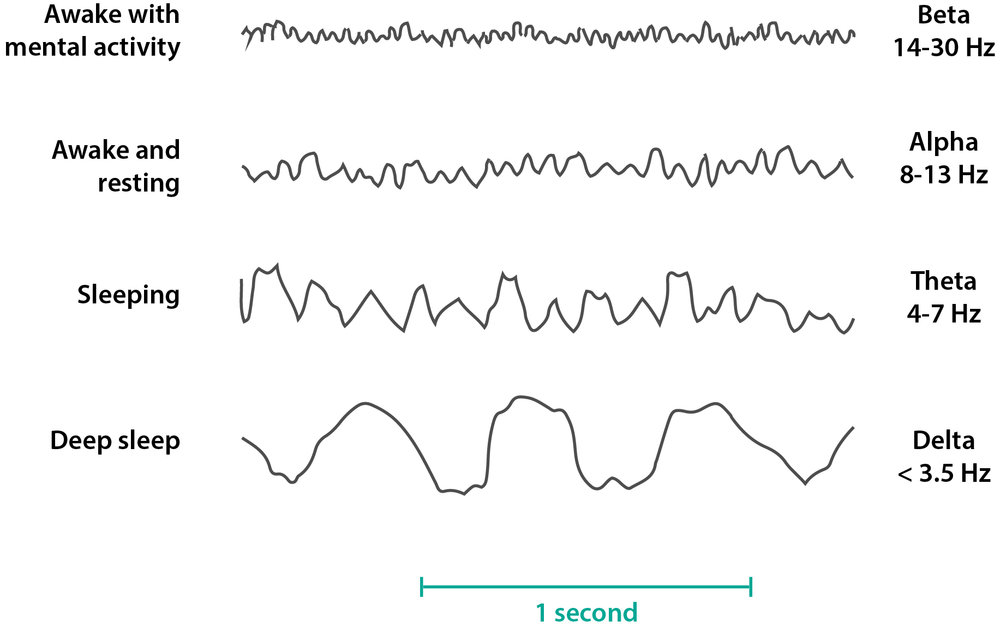
\includegraphics[width=.7\textwidth]{eeg-waves-normal}
    \caption{
امواج مغزی یا سـيگنال‌هاي
\lr{EEG}
 شامل باندهاي متفاوت فركانسي هستند كه هـر يك مرتبط با حالات فيزيكي و شناختي مختلف مي‌باشند.
         }
    \label{fig:eegNormal}
\end{figure}
 الكتروآنسفالوگرافي به حـالات مختلف مغـز (حالات استرس، هوشياري، استراحت و خـواب) حسـاس مي‌باشد. در حالت بيداري نرمال با چشم بـاز امـواج بتـا غالب مي‌باشند؛ و در حالت استراحت يا خواب آلودگي امواج آلفا افزايش مـي‌يابـد و در زمان خواب توان فعالیت نوسانی در باندهای فرکانس کمتر افزایش می‌یابد.
% و اگـر خـواب ظـاهر شـود باندهاي با فركانس كم افزايش مي‌يابد. 
 الگوی اموج مغزی منحصربه‌فرد هستند و در برخي موارد ممكن است بتوان بـر اساس فعاليت‌هاي مغزي خاص، آن‌ها را تشخيص داد.
% \cite???
%ریچارد کاتون فعالیت الکتریکی را در نیمکره مغزی خرگوش و میمون کشف کرد و یافته‌هایش را در سال ۱۸۷۵ منتشر کرد. آدولف بک در سال ۱۸۹۰، مشاهدات خود را از فعالیت الکتریکی خودبخودی مغز خرگوش و سگ منتشر کرد که شامل نوسان‌های ریتمیکی می‌شد که توسط نور تغییر یافته و به وسیله الکترودهای سطح مغز تشخیص داده شده بود. قبل از هانس برگر، ولادیمیر ولدیمویوویچ اولین  ثبت نوار مغزی
% حیوانات 
% و توانایی تحریک شده از یک سگ 
% را منتشر کرد.